\begin{figure}[ht]
\centering
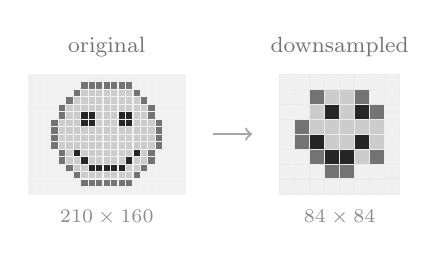
\begin{tikzpicture}[
    lbl/.style={font=\footnotesize, text=black!55},
    dimlbl/.style={font=\scriptsize, text=black!45},
]

% --- Original: 21x16 fine grid (0.095cm cells) ---
\def\cf{0.095}
\foreach \x in {0,...,20} {
    \foreach \y in {0,...,15} {
        \pgfmathsetmacro{\dist}{sqrt((\x-10)*(\x-10)+(\y-7.5)*(\y-7.5))}
        \pgfmathtruncatemacro{\inface}{\dist < 6.3 ? 1 : 0}
        \pgfmathtruncatemacro{\onedge}{(\dist >= 6.3)*(\dist < 7.2) ? 1 : 0}
        \pgfmathtruncatemacro{\feat}{(
            (\x>=7)*(\x<=8)*(\y>=9)*(\y<=10) +
            (\x>=12)*(\x<=13)*(\y>=9)*(\y<=10) +
            (\x==6)*(\y==5) + (\x==14)*(\y==5) +
            (\x==7)*(\y==4) + (\x==13)*(\y==4) +
            (\x>=8)*(\x<=12)*(\y==3)
        ) > 0 ? 1 : 0}
        \ifnum\onedge=1
            \fill[black!55, draw=black!5]
                (\x*\cf, \y*\cf) rectangle ++(\cf, \cf);
        \else\ifnum\inface=0
            \fill[black!6, draw=black!5]
                (\x*\cf, \y*\cf) rectangle ++(\cf, \cf);
        \else\ifnum\feat=1
            \fill[black!85, draw=black!5]
                (\x*\cf, \y*\cf) rectangle ++(\cf, \cf);
        \else
            \fill[black!20, draw=black!5]
                (\x*\cf, \y*\cf) rectangle ++(\cf, \cf);
        \fi\fi\fi
    }
}
\node[lbl] at ({10.5*\cf}, {16*\cf + 0.35}) {original};
\node[dimlbl, anchor=north] at ({10.5*\cf}, -0.08)
    {$210 \times 160$};

% --- Arrow ---
\draw[->, thick, black!35]
    ({21*\cf + 0.35}, {8*\cf}) -- ++(0.5, 0);

% --- Downsampled: 8x8 coarse grid (0.19cm cells, same height) ---
\def\cc{0.19}
\pgfmathsetmacro{\ox}{21*\cf + 1.2}
\pgfmathsetmacro{\oy}{0}
\foreach \x in {0,...,7} {
    \foreach \y in {0,...,7} {
        % Scaled from 21x16: center (3.8, 3.75), radius ~2.4/2.7
        \pgfmathsetmacro{\dist}{sqrt((\x-3.8)*(\x-3.8)+(\y-3.75)*(\y-3.75))}
        \pgfmathtruncatemacro{\inface}{\dist < 2.5 ? 1 : 0}
        \pgfmathtruncatemacro{\onedge}{(\dist >= 2.5)*(\dist < 2.9) ? 1 : 0}
        % Eyes and mouth scaled proportionally from 21x16
        \pgfmathtruncatemacro{\feat}{(
            (\x==3)*(\y==5) + (\x==5)*(\y==5) +
            (\x==2)*(\y==3) + (\x==5)*(\y==3) +
            (\x>=3)*(\x<=4)*(\y==2)
        ) > 0 ? 1 : 0}
        \ifnum\onedge=1
            \fill[black!55, draw=black!8]
                ({\ox + \x*\cc}, {\oy + \y*\cc}) rectangle ++(\cc, \cc);
        \else\ifnum\inface=0
            \fill[black!6, draw=black!8]
                ({\ox + \x*\cc}, {\oy + \y*\cc}) rectangle ++(\cc, \cc);
        \else\ifnum\feat=1
            \fill[black!85, draw=black!8]
                ({\ox + \x*\cc}, {\oy + \y*\cc}) rectangle ++(\cc, \cc);
        \else
            \fill[black!20, draw=black!8]
                ({\ox + \x*\cc}, {\oy + \y*\cc}) rectangle ++(\cc, \cc);
        \fi\fi\fi
    }
}
\node[lbl] at ({\ox + 4*\cc}, {8*\cc + 0.35}) {downsampled};
\node[dimlbl, anchor=north] at ({\ox + 4*\cc}, {\oy - 0.08})
    {$84 \times 84$};

\end{tikzpicture}
\caption{Downsampling. The frame is resized from $210 \times 160$
  to $84 \times 84$. Both images show the same content; the
  downsampled version has fewer, larger pixels.}
\label{fig:resize}
\end{figure}
